\documentclass[final]{beamer}
\usetheme{NTH}
\usepackage[orientation=portrait,size=a1,scale=1.4,debug]{beamerposter}
\usepackage[absolute,overlay]{textpos}
\usepackage{graphicx}
\usepackage{multicol}
\usepackage{siunitx}
\setlength{\TPHorizModule}{1cm}
\setlength{\TPVertModule}{1cm}

\title{ Computational modelling of cell-cell transport via plasmodesmata }
\author{Nathan Hughes (hughesn@nbi.ac.uk)}
\footer{
  Email: \url{hughesn@nbi.ac.uk} |
  Twitter:
  \url{NathanHughes__}}
\date{\today}

\begin{document}
\begin{frame}{}

  \begin{textblock}{28}(1,5.5)

    \begin{block}{Introduction}



    \end{block}


    \begin{block}{Results}

      \begin{multicols}{2}
        \begin{figure}[htb]
          \centering
          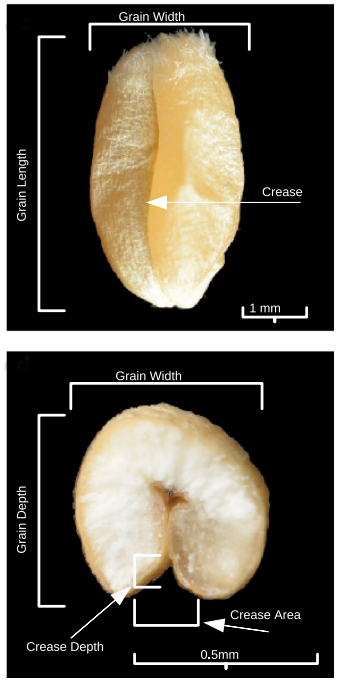
\includegraphics[width=7.3cm]{collection2.png}
          \caption{\label{fig:real} wheat grains labelled with data}
        \end{figure}

        \columnbreak

        \begin{figure}[htb]
          \centering
          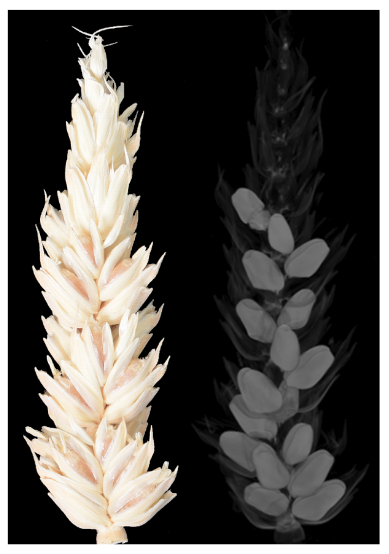
\includegraphics[width=10.5cm]{collection.png}
          \caption{\label{fig:3d} wheat Spikes original (left) and scanned (right)}
        \end{figure}

      \end{multicols}

    \end{block}

    \begin{block}{Results 2}
      \begin{multicols}{2}

      To make this research reproducible, for use in follow-up and future experiment analysis,
      I am creating a software library which acts as a specialist pipeline for handling CT-Scanner
      image data.

      \vspace{0.5cm}

      Figure:\ref{fig:flow} Illustrates a typical pipeline in which data will flow in this system.
      Primarily the process aims at taking raw uninteresting data and producing meaningful and useful
      output.

      \vspace{0.5cm}

      The pipeline will also allow a researcher to specify if they are interested in cleaning the data
      or if the outliers are of particular interest, additional options for joining in other external
      experiment information will also be possible in the final design, as flexibility is key.

        \columnbreak

        \begin{figure}[htb]
          \centering
          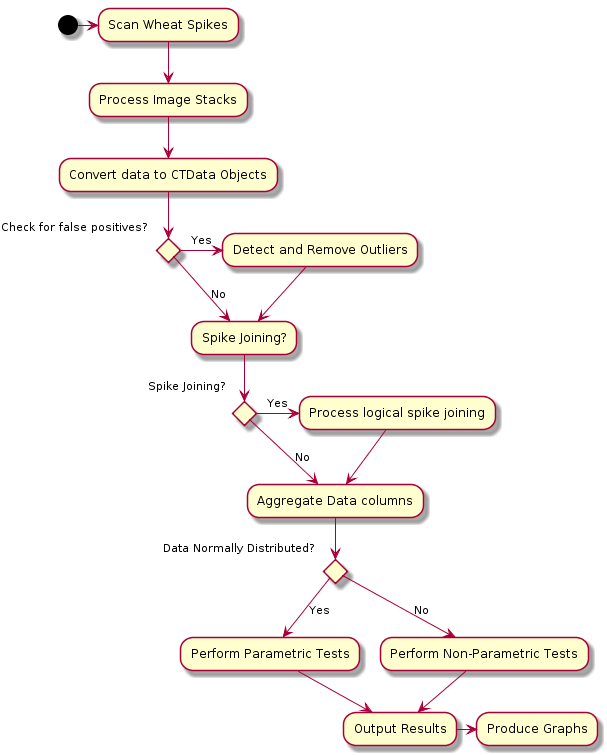
\includegraphics[width=13.5cm, height=20cm]{flow.png}
          \caption{\label{fig:flow} Data Processing Software Pipeline }
        \end{figure}

      \end{multicols}




    \end{block}

    \begin{block}{Results 3 }
      My main aim for the future is to fully implement the proposed statistical library,
      once completed I can focus on testing my outlined hypothesis.
      I will also be aiming to make use of the \textit{scipy}
      data models packages in Python.
    \end{block}


  \end{textblock}

  \begin{textblock}{28}(30.5,5.5)

    \begin{block}{Methods}


    \end{block}


    \begin{block}{Future work}

    \end{block}



    \begin{block}{Acknowledgements and Thanks}
      Thank you for the vital help and support from the following people and organisations.

      \begin{multicols}{3}

        \begin{itemize}
        \item{Prof. Richard Morris}
        \item{Dr. Christine Faulkner}

        \end{itemize}

        \columnbreak

        \begin{itemize}
        \item{Dr. Melissa Tomkins}
        \item{Morris \& Faulkner Groups}

        \end{itemize}

        \columnbreak

        \begin{itemize}
        \item{BBSRC}
        \item{NRPDTP}
        \end{itemize}

      \end{multicols}

    \end{block}

    \begin{block}{References}
      \bibliography{poster}
      \bibliographystyle{unsrt}
    \end{block}


  \end{textblock}

\end{frame}
\end{document}

%%% Local Variables:
%%% mode: latex
%%% TeX-master: t
%%% End:
